\documentclass[10pt,a4paper]{article}
\usepackage[UTF8,fontset = windows]{ctex}
\setCJKmainfont[BoldFont=黑体,ItalicFont=楷体]{华文中宋}
\usepackage{amssymb,amsmath,amsfonts,amsthm,mathrsfs,dsfont,graphicx}
\usepackage{ifthen,indentfirst,enumerate,color,titletoc}
\usepackage{tikz}
\usetikzlibrary{arrows,calc,intersections,patterns}
\usepackage[bf,small,indentafter,pagestyles]{titlesec}
\usepackage[top=1in, bottom=1in,left=0.8in,right=0.8in]{geometry}
\renewcommand{\baselinestretch}{1.65}
\newtheorem{defi}{定义~}
\newtheorem{eg}{例~}
\newtheorem{ex}{~}
\newtheorem{rem}{注~}
\newtheorem{thm}{定理~}
\newtheorem{coro}{推论~}
\newtheorem{axiom}{公理~}
\newtheorem{prop}{性质~}
\newcommand{\blank}[1]{\underline{\hbox to #1pt{}}}
\newcommand{\bracket}[1]{(\hbox to #1pt{})}
\newcommand{\onech}[4]{\par\begin{tabular}{p{.9\textwidth}}
A.~#1\\
B.~#2\\
C.~#3\\
D.~#4
\end{tabular}}
\newcommand{\twoch}[4]{\par\begin{tabular}{p{.46\textwidth}p{.46\textwidth}}
A.~#1& B.~#2\\
C.~#3& D.~#4
\end{tabular}}
\newcommand{\vartwoch}[4]{\par\begin{tabular}{p{.46\textwidth}p{.46\textwidth}}
(1)~#1& (2)~#2\\
(3)~#3& (4)~#4
\end{tabular}}
\newcommand{\fourch}[4]{\par\begin{tabular}{p{.23\textwidth}p{.23\textwidth}p{.23\textwidth}p{.23\textwidth}}
A.~#1 &B.~#2& C.~#3& D.~#4
\end{tabular}}
\newcommand{\varfourch}[4]{\par\begin{tabular}{p{.23\textwidth}p{.23\textwidth}p{.23\textwidth}p{.23\textwidth}}
(1)~#1 &(2)~#2& (3)~#3& (4)~#4
\end{tabular}}
\begin{document}
\begin{enumerate}[1.]
% 第一讲 8+3+7
\item 用适当符号($\in$, $\notin$, $=$, $\subsetneqq$)填空:$\pi$\blank{10}$\mathbf{Q}$; $\{x|x=2k+1, \ k\in \mathbf{Z}\}$\blank{10}$\{x|x=2k-1,k\in \mathbf{Z}\}$; $\{3.14\}$\blank{10}$\mathbf{Q}$; $\{y|y=x^2\}$\blank{10}$\{x|y=x^2\}$.  
\item 已知$P=\{y=x^2+1\}$, $Q=\{y|y=x^2+1, \ x\in \mathbf{R}\}$, $E=\{x|y=x^2+1, \  x\in \mathbf{R}\}$, $F=\{(x,y)|y=x^2+1, \ x\in \mathbf{R}\}$, $G=\{x|x\ge 1\}$, $H=\{x|x^2+1=0, \ x\in \mathbf{R}\}$, 则各集合间关系正确的有\blank{50}. (答案可能不唯一)\\
(A) $P=F$   (B) $Q=E$   (C) $E=F$   (D) $Q\subseteq G$  (E) $H\subsetneqq P$
\item 设全集是实数集$\mathbf{R}$, $M=\{x|-2 \le x\le 2\}$, $N=\{x|x<1\}$, 则$\complement_U M\cap N=$\blank{50}.
\item 设$A=\{x|-4<x<4, \ x\in \mathbf{R}\}$, $B=(-\infty,1]\cup [3,+\infty)$, 则$\{x|x\in A, \ x\notin A\cap B  \}$=\blank{50}.
\item 设$A=\{x|x=\sqrt k, \ k\in \mathbf{N}\}$,$B=\{x|x\le 3,\ x\in \mathbf{Q}\}$, 则$A\cap B=$\blank{50}.
\item 设全集$U=\{2,3,a^2+2a-3\}$, 集合$A=\{|2a-1|,2\}$, $\complement_U A=\{5\}$, 则实数$a=$\blank{50}.
\item (1) 设$M=\{y|y=x^2, x\in \mathbf{R}\}$, $N=\{x|x=t,\ t\in \mathbf{R}\}$, 则$M\cap N=$\blank{50}.\\
(2) 设$M=\{(x,y)|y=x^2,\ x\in \mathbf{R}\}$, $N=\{(t,x)|x=t,\ t\in \mathbf{R}\}$, 则$M\cap N=$\blank{50}.
\item 设全集$U=\{1,2,3,4\}$, $\complement_U A\cap B=\{3\}$, $A\cap \complement_U B=\{2\}$, $\complement_U A\cup \complement_U B=\{2,3,4\}$, 则$\complement_U A\cap \complement_U B=$\blank{50}.
\item 集合$C=\{x|x=\dfrac k2\pm \dfrac14, \ k\in \mathbf{Z}\},D=\{x|x=\dfrac k4,\ k\in \mathbf{Z}\}$, 试判断$C$与$D$的关系, 并证明.
\item 集合$A=\{x|x^2+4x=0\}$, $B=\{x|x^2+2(a+1)x+a^2-1=0,\ x\in \mathbf{R}\}$.\\
(1) 若$A\cap B=A$, 求实数$a$的取值范围;\\
(2) 若$A\cup B=A$, 求实数$a$的取值范围.
\item 若集合$A=[2,3]$, 集合$B=[a,2a+1]$.\\
(1) 若$A\subsetneqq B$, 求实数$a$的取值范围;\\
(2) 若$A\cap B\ne \varnothing$, 求实数$a$的取值范围.
\item 设全集$U=\mathbf{R}$, 集合$A=\{x|f(x)=0\}$, $B=\{x|g(x)=0\}$, $C=\{x|h(x)=0, \ x\in \mathbf{R}\}$, 则方程$\dfrac{f^2(x)+g^2(x)}{h(x)}=0$的解集是\blank{50}(用$U,A,B,C$表示).
\item (1) 已知集合$A=\{y|y=x^2, \ x\in \mathbf{R}\}, B=\{y|y=4-x^2, \ x\in \mathbf{R}\}$, 则$A\cap B=$\blank{50}.\\
(2) 已知集合$A=\{(x,y)|y={x^2},\ x\in \mathbf{R}\}$, $B=\{(x,y)|y=4-x^2, \ x\in \mathbf{R}\}$, 则$A\cap B=$\blank{50}.
\item 设$m\in \mathbf{R}$, 已知$A=\{x|x^2-3x+2=0\}$, $B=\{x|mx+1=0\}$, 且$B\subsetneqq A$, 则$m=$\blank{50}.
\item (1) 集合$A$满足$\{1\}\subseteq A \subsetneqq \{1,2,3,4\}$, 则满足条件的集合$A$有\blank{50}个.
(2) 若$A\cup B=\{1,2\}$, 将满足条件的集合$A$, $B$写成有序集合对$(A,B)$, 则有序集合对$(A,B)$有\blank{50}个.
\item 已知$A=\{x|x^2-3x+2=0\}$, $B=\{x|x^2-ax+a=0, \ x\in \mathbf{R}\}$, 若$B\subsetneqq A$, 求满足题意的实数$a$.
\item 设集合$A=\{x|x^2+px+1=0,\ x\in \mathbf{R}\}$, 若$A\cap \mathbf{R}^+=\varnothing$. 求实数p的取值范围.
\item 设函数$f(x)=\lg (\dfrac2{x+1}-1)$的定义域为集合$A$, 函数$g(x)=\sqrt{1-|x+a|}$的定义域为集合$B$.\\
(1) 当$a=1$时, 求集合$B$.\\
(2) 问: $a\ge 2$是$A\cap B=\varnothing$的什么条件(在``充分非必要条件、必要非充分条件、充要条件、既非充分也非必要条件''中选一)?并证明你的结论.

% 第二讲 8+3+10

\item 如图, $U$为全集, $M,P,S$是$U$的三个子集, 则阴影部分所表示的集合是\bracket{20}.
\fourch{$(M\cap P)\cap S$}{$(M\cap P)\cup S$}{$(M\cap P)\cap \complement_U S$}{$(M\cap P)\cup \complement_U S$}
\begin{center}
    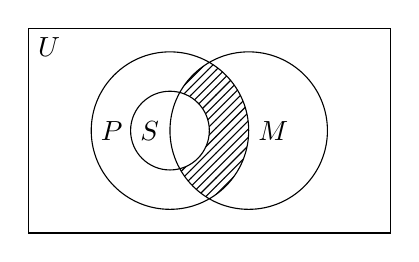
\begin{tikzpicture}
        \begin{scope}
            \clip (1,0) circle (1);
            \begin{scope}[even odd rule]
                \clip (0,0) circle (1) (0,0) circle (0.5);
                \filldraw [pattern = {north east lines}] (-2,-2) rectangle (2,2);
            \end{scope}
        \end{scope}
        \draw (0,0) circle (1) (1,0) circle (1) (0,0) circle (0.5);
        \draw (-1.8,-1.3) rectangle (2.8,1.3);
        \draw (-1.8,1.3) node [below right] {$U$} (-1,0) node [right] {$P$} (-0.5,0) node [right] {$S$} (1,0) node [right] {$M$};
    \end{tikzpicture}
\end{center}
\item 设集合$A=\{5,\log_2(a+3)\}$, $B=\{a,b\}$, 若$A\cap B=\{2\}$, 则$A\cup B=$\blank{50}.
\item 设集合$A\cap \{-2,0,1\}=\{0,1\}$, $A\cup \{-2,0,2\}=\{-2,0,1,2\}$, 则满足上述条件的集合$A$的个数为\blank{50}个.
\item 若集合$A=\{x|x\le 2\}$, $B=\{x|x\ge a\}$, 满足$A\cap B=\{2\}$, 则实数$a=$\blank{50}.
\item 若集合$M=[a-1,a+1]$, $N=(-\infty,-1)\cup [2,+\infty)$, 且$M\cap N=\varnothing$, 则实数$a$的取值范围为\blank{50}.
\item 集合$A=\{(x,y)|x^2+y^2=25\}$, $B=\{(x,y)|x=3y=4\}$, 则$A\cap B$的子集个数是\blank{50}个.
\item 已知集合$M=\{x|x=3m+1, \ m\in \mathbf{Z}\}$, $N=\{y|y=3m+2, \ m\in \mathbf{Z}\}$, 若$x_0\in M$, $y_0\in N$, 则$x_0y_0$与集合$M,N$的关系是\bracket{20}.
\twoch{$x_0y_0\in M$但$x_0y_0$$\notin N$}{$x_0y_0\in N$但$x_0y_0\notin M$}{$x_0y_0\notin M$且$x_0y_0\notin N$}{$x_0y_0$$\in M$且$x_0y_0\in N$}
\item 若$A=\{x|x=2n,\ n\in \mathbf{Z}\}$, $B=\{x|x=4m,\ m\in \mathbf{Z}\}$, 求证:$B\subsetneqq A$.
\item 设常数$a\in \mathbf{R}$, 集合$A=\{x|\dfrac{3-2x}{x-1}+1 \ge 0, \ x\in \mathbf{R}\}$, $B=\{x|2ax<a+x, \ x\in \mathbf{R} \}$.若$A\cup B=B$, 求$a$的取值范围.
\item 设常数$m\in \mathbf{R}$, $A=\{(x,y)|x^2+mx-y+2=0,\ x\in \mathbf{R}\}$, $B=\{(x,y)|x-y+1=0, x\in M\}$, 且$A\cap B\ne\varnothing$.\\
(1) 若$M=\mathbf{R}$, 求实数$m$的取值范围;\\
(2) 若$M=(\dfrac13,2]$, 求实数$m$的取值范围.
\item 设常数$k\in \mathbf{R}$, 关于$x$的不等式组$\begin{cases} x^2-x-2>0, \\ 2x^2+(2k+5)x+5k<0 \end{cases}$ 整数解的集合为$\{-2\}$, 求实数$k$的取值范围.
\item 设$A=\{(x,y)|y=-4x+6,\ x\in \mathbf{R}\}, B=\{(x,y)|y=5x-3,\ x\in \mathbf{R}\}$, 则$A\cap B=$\blank{50}.
\item 已知$M=\{a|\dfrac6{5-a}\in \mathbf{N}, \ a\in \mathbf{Z}\}$, 则用列举法表示$M=$\blank{50}.
\item 定义集合运算: $A\odot B=\{z|z=xy(x+y), \ x\in A, \ y\in B \}$, 设集合$A=\{0,1\}$, $B=\{2,3\}$, 则集合$A\odot B$的所有元素之和为\blank{50}.
\item 已知全集$U=\mathbf{R}$, $A=\{-1\}$, $B=\{x|\lg (x^2-2)=\lg x\}$, 则\bracket{20}
\fourch{$A\subseteq B$}{$A\cup B=\varnothing$}{$A\supseteq B$}{$(\complement_U A)\cap B=\{2\}$}
\item 集合$A=\{(x,y)|y=|x|+1\}$, $B=\{(x,y)|y=\dfrac12x+a\}$, 若$A\cap B=\varnothing$, 则$a$的取值范围是\blank{50}.
\item 调查某班$50$名学生, 音乐爱好者有$40$人, 体育爱好者有$24$人, 则两方面都爱好的人数最少\blank{50}人, 最多\blank{50}人.
\item 已知集合$A=\{x|ax^2-3x+2=0\}$至多有一个元素, 则$a$的取值范围是\blank{50}; 若至少有一个元素, 则$a$的取值范围是\blank{50}.
\item 设含有三个实数的集合既可以表示为$\{a,\dfrac ba,1\}$, 又可以表示为$\{a^2,a+b,0\}$, 那么$a+b=$\blank{50}.
\item 设$f(x)=x^2-12x+36$, $A=\{a|1\le a\le 10, \ a\in \mathbf{N}\}$, $B=\{b|b=f(a),\ a\in A\}$, 又设$C=A\cap B$. 求集合$C$.
\item 设常数$m\in \mathbf{R}$, $A=\{(x,y)|y=-x^2+mx-1,\ x\in \mathbf{R}\}$, $B=\{(x,y)|x+y=3,\ x\in M\}$, 且$A\cap B$的子集有两个.\\
(1) 若$M=\mathbf{R}$, 求实数$m$的值;\\
(2) 若$M=[0,3]$, 求实数$m$的取值范围.

% 第三讲 8+3+8

\item 填写下列命题的否定形式:\\
(1) $m\le 0$或$n>0$: \blank{200};\\
(2) 空间三条直线$l,m,n$两两相交: \blank{200};\\
(3) 复数$z_1,z_2,z_3$中至多一个为纯虚数: \blank{200}.
\item 已知$a,b$是整数, 写出命题``若$ab$为偶数, 则$a+b$为偶数''的逆命题、否命题、逆否命题, 并判断所写命题的真假.\\
逆命题:\blank{200}, 真假: \blank{20};\\
否命题:\blank{200}, 真假: \blank{20};\\
逆否命题:\blank{200}, 真假: \blank{20}.
\item 设甲是乙的充分非必要条件, 乙是丙的充要条件, 丁是丙的必要非充分条件, 则丁是甲的() 
\twoch{充分非必要条件}{必要非充分条件}{充要条件}{既非充分又非必要条件}
\item 若$A$是$B$的必要非充分条件, 则$\overline{A}$是$\overline{B}$的\blank{50}条件.  
\item 下列各组命题中互为等价命题的是\bracket{20}.
\twoch{$A\subseteq B$与$A\cup B=B$}{$x\in A$且$x\in B$与$x\in A\cup B$}{$a\in A\cap B$与$a\in A$或$a\in B$}{$m\in A\cap B$与$m\in A\cup B$}
\item 填空(在``充分不必要''、``必要不充分''、``充要''、``既不充分也不必要''中选一种作答):\\
(1) ``$\alpha \ne \beta$''是$\cos \alpha \ne \cos \beta$''的\blank{50}条件;\\
(2) 在$\triangle ABC$中, ``$A=B$''是``$\sin A=\sin B$''的\blank{50}条件.
\item ``$a>0b>0$''的一个必要非充分条件是\bracket{20}.
\fourch{$a>0$}{$b>0$}{$a>0b>0$}{$a,b\in \mathbf{R}$}
\item ``函数$f(x)\ (x\in \mathbf{R})$存在反函数''是``函数$f(x)$在$\mathbf{R}$上为增函数''的\bracket{20}.
\twoch{充分而不必要条件}{必要而不充分条件}{充分必要条件}{既不充分也不必要条件}
\item 填空: (填``充分不必要''、``必要不充分''、``充要''、``既不充分也不必要'')\\ 
(1) 对于实数$x,y$, $p$: $xy>1$且$x+y>2$是$q$: $x>1$且$y>1$的\blank{50}条件;\\
(2) 对于实数$x,y$, $p$: $x+y\ne 8$是$q$: $x\ne 2$或$y\ne 6$的\blank{50}条件;\\
(3) 已知$x,y\in \mathbf{R}$, $p$: $(x-1)^2+(y-2)^2=0$是$q$: $(x-1)(y-2)=0$的\blank{50}条件;\\
*(4) 设$x,y\in \mathbf{R}$, 则``$x^2+y^2<2$''是``$|x|+|y|\le \sqrt2$''的\blank{50}条件; 又是``$|x|+|y|<2$''的\blank{50}条件; 又是``$|x|<\sqrt2$且$|y|<\sqrt2$''的\blank{50}条件.\\
(5) 设$a_1,b_1,c_1,a_2,b_2,c_2$均为非零实数, 方程$a_1x^2+b_1x+c_1=0$和方程$a_2x^2+b_2x+c_2=0$的实数解集分别为$M$和$N$, 则``$\dfrac{a_1}{a_2}=\dfrac{b_1}{b_2}=\dfrac{c_1}{c_2}$''是``$M=N$''的\blank{50}条件.
\item (1) 是否存在实数$m$, 使得$2x+m<0$是${x^2}-2x-3>0$的充分条件? 说明理由.\\
(2) 是否存在实数$m$, 使得$2x+m<0$是$x^2-2x-3>0$的必要条件? 说明理由.
\item 已知关于$x$的实系数二次方程$a x^2 +bx+c=0\ (a>0)$, 分别求下列命题的一个充要条件:\\
(1) 方程有一正根, 一根是零;\\
(2) 两根都比$2$小.
\item 设$a,b\in \mathbf{R}$, 写出命题``若$a+b>0$且$ab>0$, 则$a>0$且$b>0$''的逆否命题.
\item 填空(填``充分不必要''、``必要不充分''、``充要''、``既不充分也不必要''):\\
(1) 若$x,y\in \mathbf{R}$, 则$x^2+y^2 \ne 0$是``$x,y$不全为零''的\blank{50}条件;\\
(2) 若$x,y$$\in \mathbf{R}$, 则``$xy>0,x+y>0$''是``$x>0,y>0$'' 的\blank{50}条件;\\
(3) 设$a,b\in \mathbf{R}$, 则``$|a|+|b|=|a+b|$''是``$ab=0$''的\blank{50}条件;\\   
(4) 若$a,b,c$是常数, 则``$a>0$且$b^2-4ac<0$''是``对任意$x\in \mathbf{R}$, 有$ax^2+bx+c>0$''的\blank{50}条件;\\
(5) 设$a,b\in \mathbf{R},$则$b=\tan a$是$a=\arctan b$的\blank{50}条件.
\item 已知$x,y\in \mathbf{R}$, 有如下四个命题: \textcircled{1} $x^2+y^2<1$; \textcircled{2} $|x|+|y|<1$; \textcircled{3} $|x|<1$且$y|<1$; \textcircled{4} $|x+y|<1$. 则\blank{50}是\blank{50}的充分非必要条件(答案可能不唯一).
\item 使不等式$2x^2-5x-3\ge 0$成立的一个充分不必要条件是\bracket{20}. 
\fourch{$x<0$}{$x\ge 0$}{$x\in \{-1,3,5\}$}{$x\le \dfrac12$或x$\ge 3$}
\item 已知$\alpha$:``$x\ge a$'', $\beta$:``$|x-1|\le 1$'', 若$\alpha$是$\beta$的必要非充分条件, 则实数$a$的取值范围是\blank{50}.
\item 命题甲: 关于$x$的方程$x^2+x+m=0$有两个相异的负根; 命题乙: 关于$x$的方程$4x^2+x+m=0$无实根, 若这两个命题有且只有一个是真命题, 求实数$m$的取值范围.
*\item 已知$P=\{x|x^2-8x-20 \le 0\}$, $S=\{x||x-a|\le m\}$, 求实数$a,m$的值, 使得``$x\in P$''是``$x\in S$''的充要条件.
*\item 设$f(x)=ax^2+x+a$, 写出一个$a$的值,\\
(1) 使$f(x)>0\ (x\in \mathbf{R})$恒成立;\\
(2) 使$f(x)>0\ (x\in \mathbf{R})$恒不成立;\\
(3) 使$f(x)>0\ (x\in \mathbf{R})$不恒成立. 

% 第四讲 8+3+9

\item 命题(1) $a>b\Rightarrow ac^2>bc^2$;   (2) $ac^2>bc^2\Rightarrow a>b$;     (3) $a>b\Rightarrow \dfrac 1a<\dfrac 1b$; (4) $a<b<0, \ c<d<0\Rightarrow ac>bd$;   (5) $\sqrt[n]a>\sqrt[n]b\Rightarrow a>b \ (n\in \mathbf{N}^*)$;    (6) $a+c<b+d\Leftrightarrow \begin{cases} a<b, \\ c<d; \end{cases}$ (7) $a<b<0\Rightarrow a^2>ab>b^2$. 其中真命题的序号是\blank{50}.
\item 已知$a,b\in \mathbf{R}$, 则$ab(a-b)<0$成立的一个充要条件是\bracket{20}.
\fourch{$\dfrac 1a>\dfrac 1b>0$}{$\dfrac 1a<\dfrac 1b$}{$0<\dfrac 1a<\dfrac 1b$}{$\dfrac 1a>\dfrac 1b$}
\item ``$\begin{cases} 2<x+y<4, \\ 0<xy<3 \end{cases}$''是``$\begin{cases} 2<x<3, \\ 0<y<1 \end{cases}$''的\blank{50}条件.
\item 下列函数中, 最小值为$2$的函数有\blank{50}.\\
(1) $y=x+\dfrac 1x, \ x\in (0,+\infty)$; (2) $y=x+\dfrac 1x,\ x\in (1,+\infty)$;    (3) $y=\dfrac{x^2+3}{\sqrt{x^2+2}}$;    (4)$y=\log_3x+\log_x3$.
\item $z=(x+y)(\dfrac 1x+\dfrac 1{4y}), \ (x,y>0)$的最小值是\blank{50}.
\item 若正实数$a,b$满足$a+b=1$, 则\bracket{20}.
\fourch{$\dfrac 1a+\dfrac 1b$的最大值是$4$}{$ab$的最小值是$\dfrac 14$}{$\sqrt a+\sqrt b$有最大值$\sqrt 2$}{$a^2+b^2$有最小值$\dfrac{\sqrt 2}2$}
\item 如果$0<a<b$, $t>0$, 设$M=\dfrac ab$, $N=\dfrac{a+t}{b+t}$, 那么\bracket{20}.
\twoch{$M>N$}{$M<N$}{$M=N$}{$M$与$N$的大小随$t$的变化而变化}
\item 将一根铁丝切割成三段做一个面积为$2$平方米、形状为直角三角形的框架, 则至少需要\blank{50}米的铁丝(不计损失, 精确到$0.1$米).
\item (1) 比较$1+a^2$与$\dfrac 1{1-a}$的大小;\\
(2) 设$a>0,\ a\ne 1$, $t>0$, 比较$\dfrac 12\log_at$和$\log_a\dfrac{t+1}2$的大小, 证明你的结论.
\item 已知$x,y\in \mathbf{R}^+$且$x+y=4$, 求$\dfrac 1x+\dfrac 2y$的最小值. 某学生给出如下解法: 由$x+y=4$得, $4\ge 2\sqrt{xy}$\textcircled{1}, 即$\dfrac 1{\sqrt{xy}}\ge \dfrac 12$\textcircled{2}, 又因为$\dfrac 1x+\dfrac 2y\ge 2\sqrt{\dfrac 2{xy}}$\textcircled{3}, 由\textcircled{2}\textcircled{3}得$\dfrac 1x+\dfrac 2y\ge \sqrt 2$\textcircled{4}, 即所求最小值为$\sqrt 2$\textcircled{5}.请指出这位同学错误的步骤, 并给出正确的解法.
\item 已知$x,y\in \mathbf{R}^+, \ xy=x+y+1$, 求$x+y$的取值范围(试用两种方法求解).
\item 设$a,b\in \mathbf{R}$, 若$a-|b|>0$, 则下列不等式中正确的是\bracket{20}.
\fourch{$b-a>0$}{$a^3+b^3<0$}{$b+a>0$}{$a^2-b^2<0$}
\item 已知$0<x<y<a<1$, 则\bracket{20}.
\fourch{$\log_a(xy)<0$}{$0<\log_a(xy)<1$}{$1<\log_a(xy)<2$}{$\log_a(xy)>2$}
\item 设$a>1>b>-1$, 则下列不等式中恒成立的是\bracket{20}.
\fourch{$\dfrac 1a<\dfrac 1b$}{$\dfrac 1a>\dfrac 1b$}{$a>b^2$}{$a^2>2b$}
\item 若$1<a<3$, $-4<b<2$, 则$\dfrac 12a-b$的取值范围是\blank{50}.
\item 已知$x,y\in \mathbf{R}^+$, 且$x+4y=1$, 则$x\cdot y$的最大值为\blank{50}.
\item 函数$y=\log_a(x+3)-1 \ (a>0, \ a\ne 1)$的图像恒过定点$A$, 若点$A$在直线$mx+ny+1=0$上, 其中$mn>0$, 则$\dfrac 1m+\dfrac 2n$的最小值为\blank{50}.
\item *如果正数$a,b,c,d$满足$a+b=cd=4$, 那么\bracket{20}.
\onech{$ab\le c+d$且等号成立时, $abcd$的取值唯一}{$ab\ge c+d$且等号成立时, $abcd$的取值唯一}{$ab\le c+d$且等号成立时, $abcd$的取值不唯一}{$ab\ge c+d$且等号成立时, $abcd$的取值不唯一}
\item (1) 设$x<2$, 则$2x+\dfrac 8{x-2}$有最\blank{50}值是\blank{50}, 此时$x=$\blank{50};\\
(2) 设$0<x<\sqrt 2$, 则$x\sqrt{4-2{x^2}}$的最大值是\blank{50}, 此时$x=$\blank{50}.
\item 在等差数列$\{a_n\}$和等比数列$\{b_n\}$中, $a_1=b_1>0$, $a_3=b_3>0$, $a_1\ne a_3$, 试比较$a_5$与$b_5$的大小.

% 第五讲 8+3+8
\item 下列不等式中解集为$\mathbf{R}$的是\bracket{20}.
\fourch{$x^2-6x+9>0$}{$4x^2+12x+9<0$}{$3x^2-x+2>0$}{$3x^2-x+2<0$}
\item 不等式$(x-1)^2(2-x)\le 0$的解集是\blank{50}; $(x-1)^2(2-x)>0$的解集是\blank{50}.
\item 已知关于$x$的不等式$x^2+ax+b<0$的解集为$(-1,2)$, 则$a+b=$\blank{50}.
\item 不等式$-1<x^2+2x-1\le 2$的解集是\blank{50}.
\item 用一根长为$100$米的绳子能否围成一个面积大于$600$平方米的矩形?\blank{50}(用``能''或``不能''填空).
\item 已知关于$x$的不等式$ax^2-bx+c>0$的解集是$(-\dfrac 12,2)$, 对于$a,b,c$有以下结论: \textcircled{1} $a>0$; \textcircled{2} $b>0$; \textcircled{3} $c>0$; \textcircled{4} $a+b+c>0$; \textcircled{5} $a-b+c>0$. 其中正确的序号有\blank{50}.
\item 若关于$x$的不等式$(a-2)x^2+2(a-2)x-4<0$对一切$x\in \mathbf{R}$成立, 则实数$a$的取值范围是\blank{50}.
\item 已知关于$x$的不等式$(2a-b)x+a-5b>0$的解集是$(-\infty,\dfrac{10}7)$, 则关于$x$的不等式$ax>b$的解集是\blank{50}.
\item 已知关于$x$的不等式$ax^2+bx+c>0$的解集为$\{x|2<x<4\}$, 求关于$x$的不等式$cx^2+bx+a<0$的解集.
\item 解关于$x$的不等式: $(ax+4)(x-1)>0$($a\in \mathbf{R}$).
\item 已知$f(x)=x^2+2(a-2)x+4$.\\
(1) 如果对一切$x\in \mathbf{R}$, $f(x)>0$恒成立, 求实数$a$的取值范围;\\
(2) 如果对$x\in [-3,1]$, $f(x)>0$恒成立, 求实数$a$的取值范围.
\item 不等式$-6x^2-x+2\le 0$的解集是\blank{50}.
\item 解关于$x$的不等式 $x^2-3(a+1)x+2(3a+1)\le 0$($a\in \mathbf{R}$).
\item 解关于$x$的不等式组: $\begin{cases} ax>-1, \\ x+a>0 \end{cases}$($a\in \mathbf{R}$).
\item 若关于$x$的不等式$ax^2+bx+c>0$的解集为$(-1,2)$, 求关于$x$的不等式$a(x^2+1)+b(x-1)+c>2ax$的解集.
\item 若关于$x$的不等式$(a^2-4)x^2+(a+2)x-1\ge 0$的解集为$\varnothing$, 求实数$a$的取值范围.
\item 若关于$x$的不等式$(a^2-4)x^2+(a+2)x+1\ge 0$对一切$x\in \mathbf{R}$均成立, 求实数$a$的取值范围.
\item *设$f(x)$是定义在$\mathbf{R}$上的偶函数, 在区间$(-\infty ,0)$上单调递增, 且满足$f(-a^2+2a-5)<f(2a^2+a+1)$, 求实数$a$的取值范围.
\item *已知$A=\{x|x^2-3x+2\le 0\}$, $B=\{x|x^2-(a+1)x+a\le 0\}$.\\ (1) 若$A\subsetneqq B$, 求$a$的取值范围;\\
(2) 若$B\subseteq A$, 求$a$的取值范围.

% 第六讲 8+3+10
\item 下列不等式中, 与$x^2>2$同解的不等式的序号为\blank{50}.\\
(1) $x^2+\dfrac 1{x-3}>2+\dfrac 1{x-3}$;  (2) $x^2+\sqrt{x-4}>2+\sqrt{x-4}$; (3) $x^2-(x-1)>2-(x-1)$; (4) $x^2(x-2)>2(x-2)$.
\item 不等式$\dfrac{3x+4}{5-x}\ge 6$的解集是\blank{50}.
\item 若不等式$\dfrac{2x+a}{x+b}\le 1$的解集为$\{x|1<x\le 3\}$, 则$a+b$的值是\blank{50}.
\item 不等式$(x-1)^2(2-x)(x+1)\le 0$的解集是\blank{50}.
\item 不等式$2<|x+1|<3$的解集是\blank{50}.
\item 不等式$|x-2|>9x$的解集是\blank{50}.
\item 不等式$4^{x-\frac 5x+1}\le 2$的解集是\blank{50}.
\item 不等式$\log_{\frac 14}4{x^2}>\log_{\frac 14}(3-x)$的解集是\blank{50}.
\item 解下列不等式:\\
(1) $|x-5|-|2x+3|<1$;\\
(2) $\dfrac{2x^2+x-3}{x^2+x+1}\ge 1$;\\
(3) $4^{2x}-2^{2x+2}+3<0$;\\
(4) $\log_2(x-1)<\log_4(2-x)+1$.
\item (1) 关于$x$的不等式$|x-1|-|x-2|<a^2+a-1$的解集是$\mathbf{R}$, 求实数$a$取值范围;\\
(2) 关于$x$的不等式$|x-1|-|x-2|<a^2+a-1$有实数解, 求实数$a$的取值范围.
\item *设全集$U=\mathbf{R}$, 已知关于x的不等式$|x-1|+a-1>0$($a\in \mathbf{R}$)的解集为$A$, 若$\complement_U A\cap \mathbf{Z}$恰有$3$个元素, 求$a$的取值范围.
\item 不等式$|\dfrac x{1+x}|>\dfrac x{1+x}$的解集是\blank{50}.
\item 不等式$\dfrac{2x}{1-x}\le 1$的解集是\blank{50}.
\item 不等式$\dfrac{1+|x|}{|x|-1}\ge 3$的解集是\blank{50}.
\item 设函数$f(x)=\begin{cases} 2^{-x}-1, & x\le 0, \\ x^{\frac 12}, & x>0, \end{cases}$ 若$f(x_0)>1$, 则$x_0$的取值范围是\blank{50}.
\item 已知$a>0$且$a\ne 1$, 关于$x$的不等式$a^x>\dfrac 12$的解集是$(-\infty ,1)$, 则$a=$\blank{50}.
\item 关于$x$的不等式$\log_{\frac 12}(x-\dfrac 1x)>0$的解集是\blank{50}.
\item 若不等式$|3x-b|<4$的解集中的整数有且仅有$1$, $2$, $3$, 则$b$的取值范围为\blank{50}.
\item 已知关于$x$的不等式$\dfrac{ax-5}{x^2-a}<0$的解集为$M$.\\
(1) 当$a=5$时, 求集合$M$;\\
(2) 若$2\in M$且$5\notin M$, 求实数$a$的取值范围.
\item (1) 对任意实数$x$, $|x-1|-|x+3|>a$恒成立, 求实数$a$的取值范围;\\
(2) *对任意实数$x$, $|x-1|-|x+3|>a$恒不成立, 求实数$a$的取值范围.
\item (1) 若关于$x$的不等式$x^2-kx+1>0$的解集为$\mathbf{R}$, 求实数$k$的取值范围;\\
(2) *若关于$x$的不等式$x^2-kx+1>0$在$[1,2]$上有解, 求实数$k$的取值范围.

%第七讲 0+3+7
\item 已知$a,b\in \mathbf{R}^+$, 求证: $\dfrac a{\sqrt b}+\dfrac b{\sqrt a}\ge \sqrt a+\sqrt b$.
\item 已知$x,y\in \mathbf{R}$, 求证: $x^2+y^2+1\ge x+y+xy$.
\item 已知$a,b\in \mathbf{R}^+$且$a\ne b$, 求证: $|a^3+b^3-2ab\sqrt{ab}|>|a^2b+ab^2-2ab\sqrt{ab}|$.
\item 已知$0<a<1$ ,$0<b<1$, $0<c<1$, 求证: $(1-a)b,(1-b)c,(1-c)a$中至少有一个小于等于$\dfrac 14$.
\item $a$、$b$、$c$是互不相等的正数, 则下列不等式中不正确的序号是\blank{50}.\\
(1) $|a-b|\le |a-c|+|c-b|$; (2) ${a^2}+\dfrac 1{a^2}\ge a+\dfrac 1a$; (3) $|a-b|+\dfrac 1{a-b}\ge 2$; (4) $\sqrt{a+3}-\sqrt{a+1}\le \sqrt{a+2}-\sqrt a$.
\item 已知$a>b>c>0$, 试比较$\dfrac{a-c}b$与$\dfrac{b-c}a$的大小.
\item 已知$a>0$, 试比较$a$与$\dfrac 1a$的大小.
\item 若$x,y,m,n$均为正数, 求证: $\sqrt{(m+n)(x+y)}\ge \sqrt{mx}+\sqrt{ny}$.
\item 已知$a,b,c\in \mathbf{R}^+$, 求证: $a^2b^2+b^2c^2+c^2a^2\ge a^2bc+ab^2c+abc^2$.
\item 设$f(x)=\sqrt{1+x}\ (x>0)$. 若$x_1\ne x_2$, 求证: $|f(x_1)-f(x_2)|<|x_1-x_2|$.
\item 若实数$x$、$y$、$m$满足$|x-m|>|y-m|$, 则称$x$比$y$远离$m$.\\
(1) 若$x^2-1$比$1$远离$0$, 求$x$的取值范围;\\
(2)定义: 在$\mathbf{R}$上的函数$f(x)$等于$x^2$和$x+2$中远离$0$的那个值. 求证: $f(x)\ge 1$在$\mathbf{R}$上恒成立.

%第八讲  8+3+10
\item 函数$y=\dfrac{\sqrt{2x+1}}{x-3}+(x-1)^0$的定义域为\blank{50}.
\item 若函数$y=f(x)$的定义域是$[-2,4]$, 则函数$g(x)=f(x)+f(-x)$的定义域是\blank{50}.
\item 下列各组中, 两个函数是同一个函数的组的序号是\blank{50}.\\
(1) $y=\lg x$与$y=\dfrac 12\lg {x^2}$; (2) $f(x)=2^x$, $D=\{0,1,2,3\}$与$g(x)=\dfrac 16{x^3}+\dfrac 56x+1$, $D=\{0,1,2,3\}$; \\
(3) $f(x)=x^2-2x-1$, $g(t)=t^2-2t-1$; (4) $y=\sqrt{x^2}-1$, $y=\sqrt[3]{x^3}-1$.
\item 已知函数$f(x)=6+5x-x^2$, 函数$g(x)=\dfrac {1}{\sqrt{x^2-5x-6}}$, 则$f(x)\cdot g(x)=$	\blank{50}.
\item 函数$y=f(x)$满足对于任意$x>0$, 恒有$f(x+1)=\lg x$, 则$y=f(x)$在$x>1$时的解析式为\blank{50}.
\item 函数$y=f(x)$满足对于任意$x\ne 0$, 恒有$f(x-\dfrac 1x)=x^3-\dfrac 1{x^3}$. 若存在$x_0$使得$f(x_0)=0$, 则$x_0=$\blank{50}.
\item 已知$y=f(x)$为偶函数, 且$y=f(x)$的图像在$x\in [0,1]$时的部分是半径为1的圆弧, 在$x\in [1,+\infty)$时的部分是过点$(2,1)$的射线, 如图.\\
\begin{center}
    \begin{tikzpicture}[>=latex]
        \draw [->] (-1,0) -- (4,0) node [below] {$x$};
        \draw [->] (0,-1) -- (0,3) node [left] {$y$};
        \draw (0,1) arc (90:0:1) -- (3,2);
        \draw (0,0) node [below left] {$O$};
        \draw (1,0) node [below] {$1$};
        \draw (0,1) node [left] {$1$};
        \draw [dashed] (2,0) -- (2,1) -- (0,1);
        \draw (2,0) node [below] {$2$};
    \end{tikzpicture}
\end{center}
(1) 写出函数$y=f(x)$在$x<0$时的单调性:\blank{50};\\
(2) 写出$f(f(-2))$的值:\blank{50};\\
(3) 写出方程$f(x)=\dfrac{\sqrt 3}2$的解集:\blank{50}.
\item 某工厂生产一种仪器的元件, 由于受生产能力和技术水平等因素的限制, 会产生较多次品, 根据经验知道, 次品数$p$(万件)与日产量$x$(万件)之间满足关系: $p=\begin{cases}  \dfrac{x^2}6,  &1\le x<4, \\ x+\dfrac 3x-\dfrac{25}{12}, & x\ge 4. \end{cases}$ 已知每生产$1$万件合格的元件可以盈利$20$万元, 但每产生$1$万件次品将亏损$10$万元. ($\text{实际利润}=\text{合格产品的盈利}-\text{生产次品的亏损}$), 试将该工厂每天生产这种元件所获得的实际利润$T$(万元)表示为日产量$x$(万件)的函数.
\item 设常数$a$、$b$满足$1<a<b$, 函数$f(x)=\lg(a^x-b^x)$, 求函数$y=f(x)$的定义域.
\item 如图, 用长为$l$的铁丝弯成下部为矩形, 上部为半圆形的空心框架, 若矩形底边长为$2x$, 试用解析式将此框架围成的面积$y$表示$x$的函数.
\begin{center}
    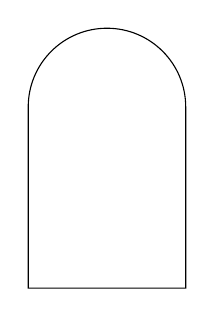
\begin{tikzpicture}
        \draw (0,0) -- (2,0) -- (2,2.3) arc (0:180:1) -- cycle;
    \end{tikzpicture}
\end{center}
\item 已知函数$f(x)=\sqrt{ax^2+x+1}$.\\
(1) 若函数$y=f(x)$的定义域为$(-\infty ,+\infty)$, 求实数$a$的取值范围;\\
(2) 若函数$y=f(x)$的值域为$[0,+\infty)$, 求实数$a$的取值范围.
\item 已知函数$f(x)=\sqrt x$, 函数$g(x)=\sqrt{1-x}-\sqrt x$, 则函数$y=f(x)+g(x)$的定义域为\blank{50}.
\item 已知函数$y=f(x)$的定义域为$[1,4]$, 则函数$y=\dfrac{f(2x)}{x-2}$的定义域是\blank{50}.
\item (1)设函数$D(x)=\begin{cases} 1, & x\in \mathbf{Q}, \\  0, &x\notin\mathbf{Q}. \end{cases}$ 令$F(x)=D(\sqrt 2x)$, 则$F(1)=$\blank{50};\\
(2) 已知函数$f(x)=\begin{cases} 2-x, & x<-2, \\ x^2, & -2\le x<1, \\ x, & x\ge 1. \end{cases}$ 若$f(x)=2$, 则$x$=\blank{50}.
\item 已知$f(x)=\begin{cases} x-2, & x>8, \\ f(x+3), & x\le 8, \end{cases}$ 则$f(2)=$\blank{50}.
\item 设常数$a\in \mathbf{R}$, $f(x)=\begin{cases}x+a, &x<a, \\ \dfrac 1x+a, & x\ge a. \end{cases}$ 若$f(2)=2$, 则$a=$\blank{50}.
\item 已知函数$f(x)=\begin{cases} \sqrt x, & x>1, \\ x, &x\le 1,  \end{cases}$ 函数$g(x)=1-\sqrt x$. 求函数$y=f(x)+g(x)$的解析式及定义域.
\item *设$D$是含数$1$的有限实数集, $f(x)$是定义在$D$上的函数, 若$f(x)$的图像绕原点逆时针旋转$\dfrac \pi6$后与原图像重合, 则在以下各项中, $f(1)$的可能取值只能是\bracket{20}
\fourch{$\sqrt3$}{$\dfrac{\sqrt{3}}2$}{$\dfrac{\sqrt{3}}3$}{$0$}
\item 设常数$p\in \mathbf{R}$, 设函数$f(x)=\log_2\dfrac{x+1}{x-1}+\log_2(x-1)+\log_2(p-x)$.\\
(1) 求$p$的取值范围以及函数$y=f(x)$的定义域;\\
(2) 若$y=f(x)$存在最大值, 求$p$的取值范围, 并求出最大值.
\item 已知$xy<0$, 且$4x^2-9y^2=36$. 问: 能否由此条件将$y$表示成$x$的函数? 若能, 求出该函数的解析式; 若不能, 说明理由.
\item 已知常数$a\in \mathbf{R}$, 函数$g(x)=\dfrac x{x+2}$, 函数$h(x)=\dfrac 1{x+a}$. 设函数$F(x)=g(x)\cdot h(x)$, $D_F$是其定义域; $f(x)=g(x)-h(x)$, $D_f$是其定义域.\\
(1) 设$a=2$, 求函数$F(x)$的值域;\\
(2) 对于给定的常数$a$, 是否存在实数$t$, 使得$f(t)=0$成立? 若存在, 求出这样的所有$t$的值; 若不存在, 说明理由;\\
(3) *是否存在常数$a$的值, 使得对于任意$x\in {D_f}\cap \mathbf{R}^+$, 有$f(x)\ge 0$恒成立? 若存在, 求出所有这样的a的值; 若不存在, 说明理由.

% 第九讲 8+3+10
\item 给定六个函数: \textcircled{1} $y=\dfrac 1x$; \textcircled{2} $y=x^2+1$; \textcircled{3} $y={x^{-\frac 13}}$; \textcircled{4} $y=2^x$; \textcircled{5} $y=\log_2x$; \textcircled{6} $y=\sqrt{x^2-1}+\sqrt{1-x^2}$.\\
在这六个函数中, 是奇函数但不是偶函数的是\blank{50}, 是偶函数但不是奇函数的是\blank{50}, 既不是奇函数也不是偶函数的是\blank{50}, 既是奇函数又是偶函数的是\blank{50}.
\item 设常数$a$、$b\in \mathbf{R}$. 若定义在$[a-2,2a]$上的$f(x)=ax^2+bx$是偶函数, 则$a=$\blank{50}, $b=$\blank{50}.
\item 设常数$a$、$b\in \mathbf{R}$. 若定义在$[a-1,a+1]$上的$f(x)=ax^2+x+b$是奇函数, 则$a=$\blank{50}, $b=$\blank{50}.
\item 若函数$f(x)=\dfrac{(x+1)(x+a)}x$为奇函数, 则实数$f(x)$\blank{50}.
\item 设函数$y=f(x)$为定义在$\mathbf{R}$上的函数, 则命题: ``$f(-1)\ne f(1)$且$f(-1)\ne -f(1)$''是命题``$y=f(x)$既不是奇函数也不是偶函数''的\blank{50}条件(填``充分不必要''、``必要不充分''、``充要''、``既不充分也不必要''之中一个).
\item 设$y=f(x)$是定义在$\mathbf{R}$上的函数, 当$x\ge 0$时, $f(x)=x^2-2x$.\\
(1) 当$y=f(x)$为奇函数时, 则当$x<0$时, $f(x)$=\blank{50};\\
(2) 当$y=f(x)$为偶函数时, 则当$x<0$时, $f(x)$=\blank{50}.
\item 设奇函数$y=f(x)$的定义域为$[-5, 5]$.若当$x\in [0,5]$时, $y=f(x)$的图像如图, 则不等式$xf(x)<0$的解是\blank{50}.
\begin{center}
    \begin{tikzpicture}[>=stealth]
        \draw [->] (-1,0) -- (6,0) node [below] {$x$};
        \draw [->] (0,-2.5) -- (0,2.5) node [left] {$y$};
        \draw (2,0) node [below] {$2$};
        \draw (5,0) node [above] {$5$};
        \draw [domain = 0:2,samples = 100] plot (\x,-\x*\x+2*\x);
        \draw [domain = 2:5,samples = 100] plot (\x, \x*\x/2-4*\x+6);
        \draw [dashed] (5,0) -- (5,-1.5);
        \draw (0,0) node [below left] {$O$};
    \end{tikzpicture}
\end{center}
\item 若定义在$\mathbf{R}$上的两个函数$y=f(x)$、$y=g(x)$均为奇函数. 设$F(x)=af(x)+bg(x)+1$.\\
(1) 若$F(-2)=10$, 则$F(2)=$\blank{50};\\
(2) 若函数$y=F(x)$在$(0,+\infty)$上存在最大值$4$, 则$y=F(x)$在$(-\infty ,0)$上的最小值为\blank{50}.
\item 判断下列函数$y=f(x)$的奇偶性:\\
(1) $f(x)=(x-1)\cdot \sqrt{\dfrac{1+x}{1-x}}$;\\
(2)$f(x)=\begin{cases} x(1-x), & x<0, \\ x(1+x),& x>0. \end{cases}$.
\item 已知函数$f(x)=x^2-2a|x-1|$, $x\in \mathbf{R}$, 常数$a\in \mathbf{R}$.\\
(1) 求证: 函数$y=f(x)$不是奇函数;\\
(2) 若函数$y=f(x)$是偶函数, 求实数$f(x)=\log_3| 2x+a |$的值.
\item 判断下列函数$y=f(x)$的奇偶性:\\
(1) $f(x)=\dfrac 1{a^x-1}+\dfrac 12$(常数$a>0$且$a\ne 1$);\\
(2) $f(x)=\dfrac{ax}{x^2-a}$(常数$a\in \mathbf{R}$).
\item 设$y=f(x)$是定义在$\mathbf{R}$上的函数, 则下列叙述正确的是\bracket{20} .
\twoch{$y=f(x)f(-x)$是奇函数}{$y=f(x)|f(-x)|$是奇函数}{$y=f(x)-f(-x)$是偶函数	}{$y=f(x)+f(-x)$是偶函数}
\item 设函数$y=f(x)$为定义在$\mathbf{R}$上的函数, 则``$f(0)\ne 0$''是``函数$y=f(x)$不是奇函数''的\bracket{20}.
\twoch{充分非必要条件}{必要非充分条件}{充要条件}{既不是充分条件, 也不是必要条件}
\item 设$y=f(x)$是定义在$\mathbf{R}$上的奇函数, 当$x<0$时, $f(x)=\lg(2-x)$, 则$x\in \mathbf{R}$时, $f(x)$=\blank{50}.
\item 判断下列函数$y=f(x)$的奇偶性, 并说明理由:\\
(1) $f(x)=x^3-\dfrac 1x$;\\
(2) $f(x)=\dfrac{|x+3|-3}{\sqrt{4-x^2}}$.
\item 根据常数$a$的不同取值, 讨论下列函数$y=f(x)$的奇偶性, 并说明理由:\\
(1) $f(a)\ge f(0)$;\\
(2) $f(x)=x|x-a|$.
\item 设函数$y=f(x)$是定义在$\mathbf{R}$上的奇函数. 若$x>0$时, $f(x)=\lg x$.\\
(1) 求方程$f(x)=0$的解集;\\
(2) 求不等式$f(x)>-1$的解集.
\item 是否存在实数$b$, 使得函数$g(x)=\dfrac{2^x}{{4^x}-b}$是奇函数? 若存在, 求$b$的值; 若不存在, 说明理由.
\item 常数$a\in \mathbf{R}$. 若函数$f(x)=\lg(10^x+1)+ax$是偶函数, 则$a=$\blank{50}.
\item 已知$y=f(x)$为定义在$\mathbf{R}$上的奇函数, $y=g(x)$为定义在$\mathbf{R}$上的偶函数, 且任意$x\in \mathbf{R}$, 都有$f(x)=g(x)+\dfrac{1}{x^2+x+1}$, 则$f(1)+g(1)=$\blank{50}.
\item 设常数$a\ne 0$. 若函数$f(x)=\lg \dfrac{x+1-2a}{x+1+3a}$. 是否存在实数$a$, 使函数$y=f(x)$为奇函数或偶函数? 若存在, 求出$a$的值, 并判断相应的$y=f(x)$的奇偶性; 若不存在, 说明理由.

%第十讲 9+2+10
\item 函数$y=\dfrac 1{x^2-4x+5}$的图像关于\bracket{20}.
\fourch{$y$轴对称}{原点对称}{直线$x=2$对称}{点$(2,1)$对称}
\item 函数$y=x+\dfrac 1{x-1}$的图像关于\bracket{20}.
\fourch{点$(1,1)$对称}{点$(-1,1)$对称}{点$(1,-1)$对称}{点$(-1,-1)$对称}
\item 若函数$y=f(x)$的定义域为$\mathbf{R}$, 且$f(x-1)=-f(3-x)$, 则$y=f(x)$的图像关于\bracket{20}.
\fourch{原点中心对称}{点$(1,0)$中心对称}{点$(2,0)$中心对称}{点$(4,0)$中心对称}
\item 设常数$a,b\in \mathbf{R}$.若函数$y=x^2+ax$在区间$[a,b]$上的图像关于直线$x=1$对称, 则$b=$\blank{50}.
\item 已知函数$y=f(x)$满足: 对于任意$x\in \mathbf{R}$, 都有$f(x+1)=-f(x)$. 若$f(1)=1$, 则$f(4)=$\blank{50}; $f(2015)=$\blank{50}.
\item 已知函数$y=f(x)$图像关于$(1,0)$对称. 若$x\le 1$时, $f(x)=x^2-1$, 则$f(x)=$\blank{50}.
\item 已知函数$y=f(x)$满足: 对于任意$x\in \mathbf{R}$, 都有$f(x+3)=f(x)$. 若$x\in [0,3)$时, $f(x)=x-1$, 则$x\in [6,9)$时, $f(x)=$\blank{50}.
\item 设常数$a\in \mathbf{R}$.已知函数$y=f(x)$满足: 对于任意$x\in \mathbf{R}$, 都有$f(x-1)=f(1-x)$. 若函数$y=f(x)$图像总是关于直线$x=a$对称, 则$a$=\blank{50}.
\item 设常数$a\in \mathbf{R}$.若直线$x=2$是函数$f(x)=\log_3|2x+a|$的图像的一条对称轴, 则$a$=\blank{50}.
\item 设函数$y=f(x)$为$\mathbf{R}$上的奇函数, 且对于任意$x\in \mathbf{R}$都有$f(x+2)=-f(x)$.\\
(1) 求证: 函数$y=f(x)$为周期函数;\\
(2) 对于任意$x\in \mathbf{R}$, 求证: $f(1+x)=f(1-x)$;\\
(3) 设$0\le x\le 1$时, $f(x)=\dfrac 12x$. 求函数$y=f(x)+\dfrac 12$在$-4\le x\le 4$时的所有零点;\\
(4) 设$-1\le x\le 1$时, $f(x)=\sin x$.\\
\textcircled{1} 写出$1\le x\le 5$时, $y=f(x)$的解析式;\\
\textcircled{2} 求$y=f(x)$在$\mathbf{R}$上的解析式.
\item 常数$a$、$b\in \mathbf{R}$. 函数$f(x)=\dfrac x{\sqrt 3}+\dfrac 1{x+a}+b$的图像关于点$(1,2)$对称.\\
(1) 求$y=f(x)$的解析式;\\
(2) *若$y=f(x)$的图像关于某一条直线对称, 写出这样的一条对称轴直线的方程(无需证明).
\item 函数$y=\log_2\dfrac{2-x}{2+x}$的图像关于\bracket{20}.
\fourch{原点对称}{$y$轴对称}{直线$y=x$对称}{直线$y=-x$对称}
\item 函数$y=\log_2(2-2^x)$的图像关于\bracket{20}.
\fourch{原点对称}{$y$轴对称}{直线$y=x$对称}{直线$y=-x$对称}
\item 设常数$a$、$b\in \mathbf{R}$. 若二次函数$f(x)=ax^2+bx+1$满足: 对任意$t\in \mathbf{R}$, $f(2+t)=f(2-t)$, 则$\dfrac ba=$\blank{50}.
\item 设定义在$\mathbf{R}$上的函数$y=f(x)$的图像关于直线$x=1$对称. 若$x\ge 1$时, $f(x)=1-3^{x-1}$, 则$x<1$时, $f(x)=$\blank{50}.
\item 设函数$y=\log_2(x+3)$的图像与函数$y=f(x)$的图像关于直线$x=1$对称. \textcircled{1} $f(1)$=\blank{50}; \textcircled{2} 若$f(a)$有意义, 则$f(a)=$\blank{50}(结果用$a$的表达式表示).
\item 已知定义域为$\mathbf{R}$的函数$y=f(x)$是偶函数, 并且其图像关于直线$x=1$对称.\\
(1) 若$f(0)=1$, $f(1)=2$, 求$f(15)+2f(20)$的值;\\
(2) 设$x\in [0,1]$时, $f(x)=x^3$.\\
\textcircled{1} $1<x\le 2$时, 求$y=f(x)$的解析式;\\
\textcircled{2} $-2\le x<0$时, 求$y=f(x)$的解析式;\\
\textcircled{3} 求函数$y=f(x)-\dfrac 18$在$[-2,2]$上的所有零点;\\
\textcircled{4} 求$y=f(x)$在$\mathbf{R}$上的解析式.
\item 已知$f(x)$是定义域为$(-\infty,+\infty)$的奇函数, 满足$f(1-x)=f(1+x)$. 若$f(1)=2$, 则$f(1)+f(2)+f(3)+\cdots +f(50)=$\bracket{20}.
\fourch{$-50$}{$0$}{$2$}{$50$}
\item 已知函数$y=f(x)$对一切$u,v\in \mathbf{R}$, 都有$f(u+v)=f(u)+f(v)$.\\
(1)	求证: $y=f(x)$是奇函数;\\ 
(2) 若$f(-3)=a$, 用$a$表示$f(6)$以及$f(300)$.
\item 已知定义在$\mathbf{R}$上的函数$y=f(x)$是奇函数, 且$y=f(x)$也是以4为周期的一个周期函数.\\
(1) 若$f(1)=1$, 则$f(-1)+f(0)=$\blank{50}; $f(10)+f(11)=$\blank{50};\\
(2) *若$f(1)=0$, 则在区间$[-3,3]$上的零点的个数的最小值为\blank{50}.
\item *设定义在$\mathbf{R}$上的函数$y=f(x)$的满足: 对于任意$x\in \mathbf{R}$, 恒有$f(-x+1)=-f(x+1)$且$f(-x-1)=-f(x-1)$. 则下面命题中, 正确的命题的序号是\blank{50}.\\
\textcircled{1} 函数$y=f(x)$是偶函数; \textcircled{2} $2$是$y=f(x)$的周期; \textcircled{3} 函数$y=f(x)$图像关于$(1,0)$对称; \textcircled{4} 函数$y=f(x)$图像关于$(3,0)$对称.


% 第十一讲 10+3+10
\item 下列函数中, 在其定义域上是单调函数的序号为\blank{50}.\\
\textcircled{1} $y=\dfrac{2-x}x$; \textcircled{2} $y=x-\dfrac 1x$; \textcircled{3} $y={3^{x-1}}$; \textcircled{4} $y=ln\dfrac 1x$; \textcircled{5} $y=tanx$.
\item 函数$y=|x-1|$递减区间的是\blank{50}.
\item 函数$y=x+\dfrac 2x$($x>0$)的递减区间是\blank{50}.
\item 函数$y=(\dfrac 12)^{x^2}$的递减区间是\blank{50}.
\item 函数$y=\dfrac 1{\sqrt{x^2+2x-3}}$的递增区间是\blank{50}.
\item 设常数$a\in \mathbf{R}$.若$y=\dfrac{ax}{x+1}$在区间$(-1,+\infty)$上递增, 则$a$的取值范围是\blank{50}.
\item 设常数$a\in \mathbf{R}$.若函数$y=x^2+ax+1$在$(-\infty,2]$上递减, 则$a$的取值范围是\blank{50}.
\item 若函数$y=f(x)$, $y=g(x)$均为$\mathbf{R}$上增函数, 则下列命题中, 正确的命题的序号是\blank{50}.\\
\textcircled{1} $y=f(x)+g(x)$为增函数; \textcircled{2} $y=f(x)\cdot g(x)$为增函数; \textcircled{3} $y=f(g(x))$为增函数.
\item 若$y=f(x)$为$\mathbf{R}$上的奇函数, 且在$(-\infty,0)$上是减函数, 又$f(-2)=0$, 则$f(x)\le 0$的解集为\blank{50}.
\item 设常数$a\in \mathbf{R}$. 若函数$f(x)=\begin{cases} x+a,& x<1, \\ x^2,& x\ge 1 \end{cases}$在$\mathbf{R}$上递增, 则$a$的取值范围为\blank{50}.
\item 设函数$f(x)=\mathrm{e}^x+\dfrac 1{\mathrm{e}^x}$.\\
(1) 求证: $y=f(x)$在$\mathbf{R}$上不是增函数;\\
(2) 求证: $y=f(x)$在$[0,+\infty)$上是增函数.
\item 设常数$a\in \mathbf{R}$. 若$y=\log_{\frac 12}(x^2-ax+2)$在$[-1,+\infty)$上是减函数, 求$a$的取值范围.
\item 已知定义在区间$(-1,1)$上的函数$y=f(x)$是奇函数, 也是减函数. 若$f(1-a)+f(1-a^2)<0$, 求实数$a$的取值范围.
\item 下列函数中, 在区间$(0 ,+\infty)$上递增的函数的序号为\blank{50}.\\
\textcircled{1} $y=|x+1|$;  \textcircled{2} $y=x-\dfrac 1x$;    \textcircled{3} $y={x^{\frac 12}}$;    \textcircled{4} $y=\sqrt{1-\dfrac 1x}$; \textcircled{5} $y=\lg x$.
\item 函数$y=\log_{0.7}(x^2-3x+2)$的单调减区间为\blank{50}.
\item 已知$y=f(x)$是偶函数, 且在区间$[0,4]$上递减. 记$a=f(2)$, $b=f(-3)$, $c=f(-4)$, 则将$a,b,c$按从小到大的顺序排列是	\blank{50}.	
\item 设常数$a\in \mathbf{R}$. ``$a=1$''是``$f(x)=|x-a|$在区间$[1, +\infty)$上为增函数''的\blank{50}条件(填: ``充分不必要''、``必要不充分''、``充要''、``既不充分也不必要''之一).
\item (1) 设常数$a\in \mathbf{R}$.若函数$y=\dfrac 1{x-a}$在区间$(0,+\infty)$上单调, 则$a$的取值范围为\blank{50}.\\
(2) 设常数$k\in \mathbf{R}$.若函数$f(x)=kx^2-4x+8$在区间$[5,20]$上单调递减, 则$k$的取值范围是\blank{50}.
\item  *设$f(x)$、$g(x)$、$h(x)$是定义域为$R$的三个函数, 对于下列命题:\\
\textcircled{1} 若$f(x)+g(x)$、$f(x)+h(x)$、$g(x)+h(x)$均为增函数, 则$f(x)$、$g(x)$、$h(x)$中至少有一个是增函数;\\
\textcircled{2} 若$f(x)+g(x)$、$f(x)+h(x)$、$g(x)+h(x)$均是以$T$为周期的函数, 则$f(x)$、$g(x)$、$h(x)$均是以$T$为周期的函数, 下列判断正确的是\bracket{20}.
\twoch{\textcircled{1}和\textcircled{2}均为真命题}{\textcircled{1}和\textcircled{2}均为假命题}{\textcircled{1}为真命题, \textcircled{2}为假命题}{\textcircled{1}为假命题, \textcircled{2}为真命题}
\item 设常数$a,b\in \mathbf{R}$. 已知$f(x)=\dfrac{ax^2+1}{x+b}$是奇函数, $f(1)=5$.\\
(1) 求$a,b$的值;\\
(2) 求证: $y=f(x)$在区间$(0,\dfrac 12]$上是减函数.
\item 求证: 函数$f(x)=\dfrac 1x-\lg\dfrac{1+x}{1-x}$是奇函数, 且在区间$(0,1)$上递减.
\item 设常数$a\in \mathbf{R}$.若函数$f(x)=\log_a(2-ax)$在$[0,1]$上是减函数, 求$a$的取值范围.
\item 已知定义$\mathbf{R}$上的函数$y=f(x)$满足下面两个条件:\\
(I) 对于任意$x_1,x_2\in \mathbf{R}$, 都有$f(x_1+x_2)=f(x_1)+f(x_2)$; (II)当$x>0$时, $f(x)>0$, 且$f(1)=1$.\\
(1) 求证: $y=f(x)$是奇函数;\\
(2) 求证: $y=f(x)$在$\mathbf{R}$上是增函数;\\
(3) *解不等式$f(x^2-1)<2$.

% 第十二讲 10+3+10
\item 函数$y=x^{-\frac 32}$的定义域为\blank{50}.
\item 下列命题中, 正确的命题的序号是\blank{50}.\\
\textcircled{1} 当$\alpha =0$时, 函数$y={x^{\alpha }}$的图像是一条直线;\\
\textcircled{2} 幂函数的图像都经过(0, 0)和(1, 1)点;\\
\textcircled{3} 当$\alpha <0$且$y={x^{\alpha }}$是奇函数时, 它也是减函数;\\
\textcircled{4} 第四象限不可能有幂函数的图像.
\item 图中曲线是幂函数$y=x^n$在第一象限的图像, 已知$n$取$\pm 2$, $\pm\dfrac 12$四个值, 则相应于曲线$c_1,c_2,c_3,c_4$的$n$依次为\bracket{20}.
\begin{center}
    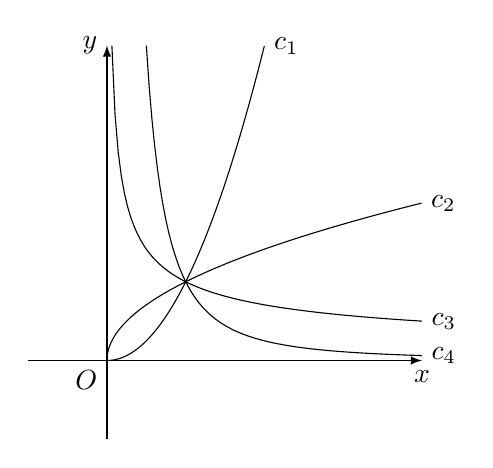
\begin{tikzpicture}[>=latex]
        \draw [->] (-1,0) -- (4,0) node [below] {$x$};
        \draw [->] (0,-1) -- (0,4) node [left] {$y$};
        \draw (0,0) node [below left] {$O$};
        \draw [domain = 0:2, samples = 100] plot (\x,\x*\x) node [right] {$c_1$};
        \draw [domain = 0:2, samples = 100] plot (\x*\x,\x) node [right] {$c_2$};
        \draw [domain = 0.0625:4, samples = 100] plot (\x, {1/sqrt(\x)}) node [right] {$c_3$};
        \draw [domain = 0.5:4, samples = 100] plot (\x, {1/\x/\x}) node [right] {$c_4$};
    \end{tikzpicture}
    \end{center}
\fourch{$-2,-\dfrac 12,\dfrac 12,2$}{$2,\dfrac 12,-\dfrac 12,-2$
}{$-\dfrac 12,-2,2,\dfrac 12$}{$2,\dfrac 12,-2,-\dfrac 12$}
\item 下列函数的图像为(A)、(B)、(C)、(D)之一, 试将正确的字母标号填在相应函数后面的横线上.
\begin{center}
    \begin{tikzpicture}[>=latex,scale = 0.5]
        \draw [->] (-3,0) -- (3,0) node [below] {$x$};
        \draw [->] (0,-3) -- (0,3) node [left] {$y$};
        \draw (0,0) node [below right] {$O$};
        \draw [domain = {-3^(1/4)}:{3^(1/4)}] plot (\x*\x*\x,\x*\x*\x*\x);
        \draw (0,-3) node [below] {(A)};
    \end{tikzpicture}
    \begin{tikzpicture}[>=latex,scale = 0.5]
        \draw [->] (-3,0) -- (3,0) node [below] {$x$};
        \draw [->] (0,-3) -- (0,3) node [left] {$y$};
        \draw (0,0) node [below right] {$O$};
        \draw [domain = {-3^(1/5)}:{3^(1/5)}] plot (\x*\x*\x,\x*\x*\x*\x*\x);
        \draw (0,-3) node [below] {(B)};
    \end{tikzpicture}
    \begin{tikzpicture}[>=latex,scale =0.5]
        \draw [->] (-3,0) -- (3,0) node [below] {$x$};
        \draw [->] (0,-3) -- (0,3) node [left] {$y$};
        \draw (0,0) node [below right] {$O$};
        \draw [domain = {0}:{3^(1/3)}] plot (\x*\x,\x*\x*\x);
        \draw (0,-3) node [below] {(C)};
    \end{tikzpicture}
    \begin{tikzpicture}[>=latex,scale = 0.5]
        \draw [->] (-3,0) -- (3,0) node [below] {$x$};
        \draw [->] (0,-3) -- (0,3) node [left] {$y$};
        \draw (0,0) node [below right] {$O$};
        \draw [domain = {3^(-3/2)}:3] plot (\x,{\x^(-2/3)}) plot (-\x,{\x^(-2/3)});
        \draw (0,-3) node [below] {(D)};
    \end{tikzpicture}
    \end{center}
(1) $y=x^\frac 32$\blank{50}; (2) $y=x^\frac 43$\blank{50}; (3) $y=x^\frac 53$\blank{50}; (4) $y=x^{-\frac 23}$\blank{50}.
\item 已知$\alpha\in \{-2,-1,-\dfrac 12,\dfrac 12,1,2,3\}$, 若幂函数$f(x)=x^\alpha$为奇函数, 且在$(0,+\infty)$上递减, 则$\alpha=$\blank{50}.
\item 函数$y=f(x)$满足两个条件:
\textcircled{1} $y=f(x)$是两个幂函数的和函数; \textcircled{2} $y=f(x)$的最小值为2, 则$y=f(x)$的解析式可以是\blank{50}.
\item 若集合$A=\{y|y={x^{\frac 13}}, \ -1\le x\le 1\}$, $B=\{y|y={x^{-\frac 12}}\}$, 则$A\cap B$等于\bracket{20}.
\fourch{$(0,1]$}{$[-1,1]$}{$\{1\}$}{$\{0,1\}$}
\item 设常数$m\in \mathbf{R}$. 若幂函数$y=(m^2-m-1)x^{m^2-2m-1}$在$(0,+\infty)$上是增函数, 则$m$的值为\blank{50}.
\item 设常数$n\in \mathbf{Z}$. 若函数$y=x^{n^2-2n-3}$的图像与两条坐标轴都无公共点, 且图像关于$y$轴对称, 则$n$的值为\blank{50}.
\item 函数$y=1-(x+2)^{-2}$可以先将幂函数$y=x^{-2}$的图像向\blank{50}平移$2$个单位, 再以\blank{50}轴为对称轴作对称变换, 最后向\blank{50}平移$1$个单位.
\item 在$f(x)=(2m^2-7m-9)x^{m^2-9m+19}$中, 当实数$m$为何值时,\\
(1) $y=f(x)$是正比例函数, 且它的图像的倾斜角为钝角?\\
(2) $y=f(x)$是反比例函数, 且它的图像在第一, 三象限?
\item 设常数$t\in \mathbf{Z}$. 已知幂函数$y=(t^3-t+1){x^{\frac 13(1+2t-t^2)}}$是偶函数, 且在区间$(0,+\infty)$上是增函数, 求整数$t$的值, 并作出相应的幂函数的大致图像.
\item 设$a\in \mathbf{R}$.\\
(1) 若$(a+2)^{\frac 23}>{(1-2a)}^{\frac 23}$, 求$a$的取值范围;\\
(2) 若$(a+2)^{-\frac 13}>(1-2a)^{-\frac 13}$, 求$a$的取值范围.
\item 已知函数: \textcircled{1} $y=\dfrac 1x$; \textcircled{2} $y=x^{\dfrac 12}$; \textcircled{3} $y=x^{-\dfrac 12}$; \textcircled{4} $y={x^{\dfrac 23}}$; \textcircled{5} $y=x^{-\dfrac 23}$, 填写分别具有下列性质的函数序号:\\ 
(1) 图像与$x$轴有公共点的:\blank{50};\\
(2) 图像关于原点对称的:\blank{50};\\
(3) 定义域内递减的:\blank{50};\\
(4) 在定义域内有反函数的:\blank{50}.
\item 函数$y=-(x+1)^{-3}$的图像可以先将幂函数$y=x^{-3}$的图像向\blank{50}平移1个单位, 再以\blank{50}轴为对称轴作对称变换.
\item 设$\alpha \in \{-3,-\dfrac 23,-\dfrac 12,-\dfrac 13,\dfrac 13,1,\dfrac 32,2\}$. 已知幂函数$y=x^{\alpha}$是奇函数, 且在区间$(0,+\infty)$上是减函数, 则满足条件的$\alpha$的值是\blank{50}.
\item 下列关于幂函数图像及性质的叙述中, 正确的叙述的序号是\blank{50}.\\
\textcircled{1} 对于一个确定的幂函数, 第二、三象限不可能同时有该幂函数的图像上的点;\\
\textcircled{2} 若某个幂函数图像过$(-1,-1)$, 则该幂函数是奇函数;\\
\textcircled{3} 若某个幂函数在定义域上递增, 则该幂函数图像必经过原点;\\
\textcircled{4} 幂函数图像不会经过点$(-\dfrac 12,8)$以及$(-8,-4)$.
\item 设$y=f(x)$与$y=g(x)$是两个不同的幂函数, 集合$M=\{x|f(x)=g(x)  \}$, 则集合$M$中的元素是\bracket{20}.
\fourch{$1$或$2$}{$1$或$3$}{$1$或$2$或$3$}{$1$或$2$或$3$或$4$}
\item 已知幂函数$y=x^{\frac qp}$($p\in \mathbf{N}^*,\ q\in \mathbf{N}^*$, $p,q$互质)的图像如图所示, 则\bracket{20}.
\begin{center}
    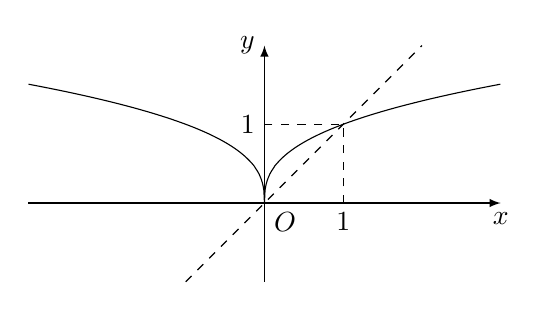
\begin{tikzpicture}[>=latex]
        \draw [->] (-3,0) -- (3,0) node [below] {$x$};
        \draw [->] (0,-1) -- (0,2) node [left] {$y$};
        \draw (0,0) node [below right] {$O$};
        \draw [dashed] (-1,-1) -- (2,2);
        \draw [domain = 0:3, samples = 400] plot (\x,{\x^(3/8)}) plot (-\x,{\x^(3/8)});
        \draw [dashed] (1,0) node [below] {$1$} -- (1,1) -- (0,1) node [left] {$1$};
    \end{tikzpicture}
\end{center}
\twoch{$p,q$均为奇数}{$p$是奇数, $q$是偶数, 且$0<\dfrac qp<1$}{$p$是偶数, $q$是奇数}{$p$是奇数, $q$是偶数, 且$\dfrac qp>1$}
\item 若$(x+1)^{-\frac 13}<(3-2x)^{-\frac 13}$, 求实数$x$的取值范围.
\item 设常数$a,b$满足$a>b>0$. 已知函数$f(x)=\dfrac{x+a}{x+b}$.
(1) 写出函数$y=f(x)$的单调性;\\
(2) 写出函数$y=f(x)$图像的一个对称中心的坐标.
\item 已知函数$f(x)=\dfrac{x^{\frac 13}-x^{-\frac 13}}5$, $g(x)=\dfrac{x^{\frac 13}+x^{-\frac 13}}5$.\\
(1) 分别计算$f(4)-5f(2)g(2)$和$f(9)-5f(3)g(3)$的值;\\
(2) 由(1)概括出涉及函数$y=f(x)$和$y=g(x)$的, 对所有不等于零的实数$x$都成立的一个等式, 并加以证明.
\item *证明第8题中的对称中心是唯一的.



 


\end{enumerate}

\end{document}